% =============================================================================
% chemistry-framework -- manuscript for Journal of Cheminformatics (BMC)
% Research article. Single column, Times, unnumbered BMC-style headings,
% structured abstract, Vancouver-style numeric references.
% Build: pdflatex main ; pdflatex main
% =============================================================================
\documentclass[10pt,a4paper]{article}

\usepackage[T1]{fontenc}
\usepackage[utf8]{inputenc}
\usepackage{lmodern}
\usepackage{mathptmx}
\renewcommand{\ttdefault}{lmtt}
\usepackage[margin=24mm,top=25mm,bottom=25mm]{geometry}
\usepackage{amsmath,amssymb}
\usepackage{graphicx}
\usepackage{booktabs}
\usepackage{array}
\usepackage{multirow}
\usepackage{xcolor}
\usepackage{url}
\usepackage{enumitem}
\usepackage{microtype}
\usepackage{setspace}
\usepackage{lineno}
\usepackage[font=small,labelfont=bf,labelsep=period,justification=justified,singlelinecheck=false]{caption}
\usepackage{titlesec}
\usepackage[hidelinks]{hyperref}

\usepackage{listings}
\lstdefinelanguage{yaml}{morecomment=[l]{\#},morestring=[b]", sensitive=true}
\lstset{
  language=yaml,
  basicstyle=\ttfamily\footnotesize,
  columns=fullflexible,
  showstringspaces=false,
  breaklines=true,
  breakatwhitespace=true,
  breakindent=1em,
  commentstyle=\itshape,
  frame=single,
  framerule=0.3pt,
  numbers=none,
  xleftmargin=3pt,
  xrightmargin=3pt,
  aboveskip=6pt,
  belowskip=6pt
}

% --- BMC-like heading style: bold, unnumbered -------------------------------
\setcounter{secnumdepth}{0}
\titleformat{\section}{\normalfont\bfseries\large}{}{0pt}{}
\titlespacing*{\section}{0pt}{14pt plus 2pt minus 2pt}{5pt}
\titleformat{\subsection}{\normalfont\bfseries\normalsize}{}{0pt}{}
\titlespacing*{\subsection}{0pt}{11pt plus 2pt minus 2pt}{3pt}
\titleformat{\subsubsection}{\normalfont\bfseries\itshape\normalsize}{}{0pt}{}
\titlespacing*{\subsubsection}{0pt}{9pt plus 1pt minus 1pt}{2pt}

\captionsetup[figure]{name=Fig.}
\captionsetup[table]{skip=4pt}

\newcommand{\framework}{\texttt{chemistry-framework}}
\newcommand{\cfg}[1]{\texttt{#1}}

\renewcommand{\arraystretch}{1.0}
\setlength{\parindent}{0pt}
\setlength{\parskip}{5pt plus 1pt minus 1pt}
\onehalfspacing

\begin{document}

% ---------------------------------------------------------------------------
% Title block
% ---------------------------------------------------------------------------
\begin{flushleft}
{\small\scshape Research article}\\[6pt]
{\LARGE\bfseries Evidence before prediction: a configuration-driven framework for testing how molecular descriptors shape property models}\\[14pt]
{\large D.~K.~N.~N.}$^{1}$\\[4pt]
{\small $^{1}$\emph{[Department, Institution, City, Country]}}\\[2pt]
{\small Correspondence: \emph{[email address]}}\\[6pt]
\end{flushleft}

\vspace{2pt}
\hrule
\vspace{10pt}

% ---------------------------------------------------------------------------
% Structured abstract
% ---------------------------------------------------------------------------
\section*{Abstract}

\noindent\textbf{Background.} When a chemist builds a machine-learning model for a molecular property, most of the attention goes to the learner: a graph neural network, a descriptor-based model, or a hybrid. In practice much of the outcome is decided earlier, by the quality of the data, by which of several hundred descriptors enter the model, and by the role those descriptors are given. These choices are usually buried in task-specific scripts, so a reader cannot tell which were tested, which were assumed, and which produced the reported score.

\noindent\textbf{Results.} We present \framework, an open-source workflow in which an experiment is declared in one validated configuration file and every run writes a record that can be replayed. We tested three hypotheses. \emph{H1, that training-partition evidence can guide descriptor choice}, is partly supported: the chosen subset had the better mean in all 20 dataset--budget cells and beat a 50-draw random control significantly in 16, but the rule ranked fourth of six selectors (mean rank 3.65). \emph{H2, that the effect of adding descriptors transfers between implementations}, holds on four of five endpoints: the framework and Chemprop v2.3.1 agreed in direction and approximate size ($+12.1\%$ versus $+19.7\%$ on FreeSolv; at most about $2\%$ elsewhere), and on ESOL one divergent run ($2.76$ RMSE) explained the disagreement: six retrainings span $0.75$--$6.12$, and bounding the descriptor inputs collapses them to $0.65$--$0.72$, where both place the effect at zero. \emph{H3, that routes and predictive roles matter but are endpoint-specific}, holds: the full 210-descriptor hybrid led on ESOL and FreeSolv, the recommender route on Lipophilicity and graph-only on BACE, while on BBBP every route lay within $0.007$ AUROC. No compact route separated from its matched random control.

\noindent\textbf{Conclusions.} Evidence from the training partition is useful for narrowing choices, but it does not name a universal winner, and a mean that hides one divergent run is unfinished evidence. Declaring the audit, the descriptor evidence, the route and the role in one configuration makes these comparisons cheap to run and possible to audit. The framework does not prescribe a better predictor; it makes the alternatives testable on the user's own data.

\vspace{6pt}
\noindent\textbf{Keywords:} Cheminformatics; molecular property prediction; feature selection; graph neural networks; QSAR; reproducibility; configuration-driven software

\vspace{4pt}
\hrule
\vspace{4pt}

\linenumbers

\section{Background}\label{sec:introduction}

A chemist who wants a model for a molecular property usually starts with a table: one row per compound, a SMILES string, and a measured value. Turning that table into a trustworthy prediction involves three decisions that are made before any model is fitted. The first is whether the data can carry the weight placed on them: are the structures valid, are they duplicated, do the labels agree, and does the training set cover the chemistry that will be predicted \cite{fourches2010trust}? The second is which of several hundred computed descriptors \cite{todeschini2009descriptors,moriwaki2018mordred} should enter the model, if any. The third is the role those descriptors should play: passed to the model as additional input, used as a fixed baseline, or used as the starting point that a graph network corrects.

In practice these three decisions are encoded in task-specific scripts. The script mixes the chemical judgement with the engineering plumbing, so a reader cannot tell which options were tested, which were assumed, and which produced the reported number. Six months later the comparison is hard to repeat exactly. The problem is not a lack of algorithms. Descriptor-based models, fingerprints, and graph neural networks \cite{gilmer2017mpnn,yang2019dmpnn,xu2019gin} are all well developed, and benchmark collections such as MoleculeNet \cite{wu2018moleculenet} and the Therapeutics Data Commons \cite{huang2021tdc} allow systematic comparisons across endpoints \cite{mayr2018largescale,jiang2021gnn,deng2023systematic}. Prior work shows that descriptor-based models can match or outperform graph models on some tasks, and that adding descriptors to a learned graph representation can help on others \cite{aouichaoui2023gcgnn,wieder2020review}. The recurring lesson is that the usefulness of a representation depends on the endpoint, the curation of the data, and the evaluation protocol, not on the model class alone.

Decisions about features are equally consequential. Quantitative structure--activity and structure--property relationship (QSAR/QSPR) guidance asks for a defined endpoint, a transparent algorithm, and a stated applicability domain \cite{oecd2007guidance,tropsha2010best,cherkasov2014qsar}. Feature selectors address part of this: filters rank descriptors by correlation or mutual information \cite{guyon2003introduction,khan2018featureselection,shahlaei2013descriptor,danishuddin2016descriptors}, while embedded methods use a fitted learner, such as Random Forest importance \cite{strobl2007bias} or sparse regression, to rank them. Every such ranking is evidence for a particular dataset, learner, and budget. It is not a universal statement about which molecular properties matter, and presenting it as one is a common source of over-claiming.

A related decision is how the selected information enters the predictor. Descriptors may be concatenated with a learned graph representation, used as a fixed linear prior learned on the training set, or used as the baseline that the graph model corrects. We call the assignment of a feature block to a task a \emph{route}, and the way its output enters the predictor a \emph{role}. These roles answer different modelling questions, yet they are usually implemented in separate scripts or frozen into a pipeline, which makes an otherwise simple comparison expensive.

Open-source software already supplies much of the infrastructure. Chemprop provides efficient directed message-passing networks \cite{heid2024chemprop,graff2026chemprop}, DeepMol and QSARtuna automate pipeline and model search \cite{correia2024deepmol,mervin2024qsartuna,dixon2016autoqsar}, QSPRpred emphasises reproducible and serialisable QSPR workflows \cite{vandenmaagdenberg2024qsprpred}, ZairaChem targets automated screening cascades \cite{turon2023zairachem}, and integrated frameworks aim at scalable molecular property prediction \cite{chen2023integrated}. General tools such as Hydra and MLflow record settings and runs \cite{yadan2019hydra,zaharia2018mlflow}. The gap addressed here is narrower and, we argue, more useful to a chemist: none of these tools makes training-partition feature evidence, descriptor recommendations, feature routes, and predictive roles explicit inside one auditable experiment record (Table~\ref{tab:positioning}).

\begin{table}[t]
\caption{Emphasis of related open-source molecular machine-learning tools, summarised from the cited publications. Entries are not exhaustive feature lists.}
\label{tab:positioning}
\centering
\footnotesize
\setlength{\tabcolsep}{4pt}
\begin{tabular}{@{}>{\raggedright\arraybackslash}p{0.15\textwidth}>{\raggedright\arraybackslash}p{0.27\textwidth}>{\raggedright\arraybackslash}p{0.27\textwidth}>{\raggedright\arraybackslash}p{0.24\textwidth}@{}}
\toprule
Tool & Primary emphasis & Feature handling & Roles of feature groups \\
\midrule
Chemprop v2 \cite{graff2026chemprop} & Efficient, modular D-MPNN training and inference & Optional extra atom-, bond-, and molecule-level features & Direct (concatenated with the learned representation) \\
DeepMol \cite{correia2024deepmol} & Automated search over preprocessing, representation, and model pipelines & Feature extraction and selection as pipeline steps & Direct model input \\
QSARtuna \cite{mervin2024qsartuna} & Automated QSAR model and hyperparameter optimisation & Choice among descriptor and fingerprint representations & Direct model input \\
QSPRpred \cite{vandenmaagdenberg2024qsprpred} & Reproducible, serialisable QSPR modelling, including proteochemometrics & Training-only variance, correlation, and Boruta \cite{kursa2010boruta} filters & Direct model input \\
This work & Auditable link between feature evidence and model configuration & Training-partition evidence scorecard, dataset audit, relevance and redundancy recommender & Direct, fixed prior, or learned residual, declared per feature block \\
\bottomrule
\end{tabular}
\end{table}

We therefore built \framework, an open-source Python package in which an experiment is declared in one plain-text configuration file. The file names the dataset, the molecular representations, the split, the model, and the role of each descriptor block; it is checked against a typed schema before any computation starts. Fig.~\ref{fig:workflow} shows the five stages a user goes through, from a table of SMILES and measured values to a saved record that another person can replay. The framework does not replace the chemist's judgement. It makes each judgement visible, testable, and cheap to change.

\begin{figure}[t]
\centering
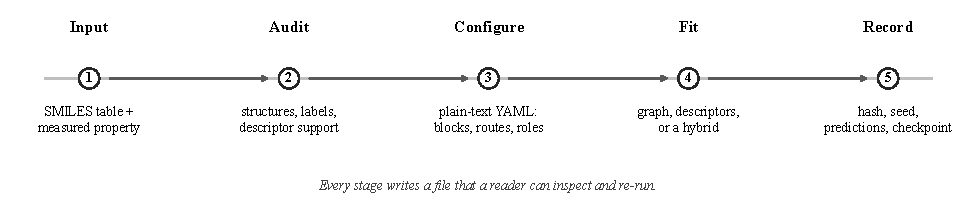
\includegraphics[width=0.98\textwidth]{figs/fig1_pipeline.pdf}
\caption{The five stages of a \framework{} experiment. A table of SMILES and measured properties is read and audited, the experiment is declared in a validated configuration file, the selected representations are fitted, and every run writes a record (configuration hash, split seed, predictions, checkpoint) that a reader can inspect and re-run. The framework changes what is explicit, not what is chemically possible.}
\label{fig:workflow}
\end{figure}

\subsection*{What this study tests}

The paper is organised around three hypotheses, stated here so that the reader can judge the results against them rather than after the fact.

\begin{description}\sloppy
\item[H1 --- Evidence is usable.] Training-partition diagnostics of descriptors, together with a transparent relevance-and-redundancy rule, carry enough information to guide descriptor choice. \emph{Prediction:} (i) descriptor subsets chosen from this evidence should beat random subsets of the same size in most dataset--budget cells tested; (ii) the rule should rank in the upper half of the selectors compared against it; and (iii) the choice should be stable across splits. \emph{Falsified if:} the evidence-based choice is indistinguishable from a random one, or if the rule ranks in the lower half of the selectors.
\item[H2 --- The descriptor effect transfers.] The effect of adding descriptors to a graph model is a property of the endpoint and the data, not of one software implementation. \emph{Prediction:} an independently written implementation (Chemprop v2.3.1, with a different encoder, featurisation and training loop) should change in the same direction and by a similar amount on most endpoints. Because the two systems differ in more than the descriptor block, agreement is evidence that the effect transfers, not a decomposition of it into architecture and features; the architecture-unconfounded estimate is the within-system contrast. \emph{Falsified if:} the two implementations disagree in sign across endpoints.
\item[H3 --- Route and role matter, but not universally.] Compact descriptor routes and alternative predictive roles change results, yet the best choice is endpoint-specific and small compared with split-to-split variation. \emph{Prediction:} no single route or role wins everywhere, and most differences should be comparable to the between-split standard deviation. \emph{Falsified if:} one configuration wins on every endpoint by a margin that exceeds the split variation.
\end{description}

Testing these hypotheses requires more than a new script. It requires the same splits, the same checkpoints, and the same evaluation rule across every model, and it requires that the comparison be reproducible by someone who did not run it. The remainder of the paper reports the design (Methods), the results for each hypothesis (Results), what they do and do not imply for a practising chemist (Discussion), and the conclusions (Conclusions). Table~\ref{tab:result-map} maps each hypothesis to its experiment and to the section and table where the evidence is reported.

\begin{table}[t]
\caption{Reading map: each hypothesis, the experiment that tests it, and where the answer is reported.}
\label{tab:result-map}
\centering
\footnotesize
\setlength{\tabcolsep}{4pt}
\begin{tabular}{@{}>{\raggedright\arraybackslash}p{0.05\textwidth}>{\raggedright\arraybackslash}p{0.26\textwidth}>{\raggedright\arraybackslash}p{0.36\textwidth}>{\raggedright\arraybackslash}p{0.23\textwidth}@{}}
\toprule
 & Hypothesis & Experiment & Reported in \\
\midrule
H1 & Training-partition evidence guides descriptor choice & Scorecard and dataset audit on five endpoints; six selectors at four budgets with a Random Forest downstream; recommended versus random subsets & Descriptor evidence and data audit; Tables~\ref{tab:selectors} and \ref{tab:hygiene}; Fig.~\ref{fig:worked} \\
H2 & The descriptor effect transfers between implementations & Graph-only and graph-plus-descriptor models in \framework{} and in Chemprop v2.3.1, on the same saved splits & Predictive performance; Tables~\ref{tab:baselines-regression} and \ref{tab:baselines-classification}; Fig.~\ref{fig:descriptor-effect} \\
H3 & Route and role matter, but the best choice is endpoint-specific & Five role configurations; a harmonised routing experiment with Spearman, mutual-information and random controls; per-split paired comparisons & Descriptor routing and predictive roles; Tables~\ref{tab:routing} and \ref{tab:ablation}; Fig.~\ref{fig:routing} \\
\bottomrule
\end{tabular}
\end{table}

\section{Results}\label{sec:results}

\subsection{Performance depends on the endpoint, not on the model class}\label{subsec:cross-task-results}

The best model depended on the task (Tables~\ref{tab:baselines-regression} and \ref{tab:baselines-classification}). The descriptor MLP and the framework direct hybrid tied for the lowest mean RMSE on ESOL ($0.623$), the framework direct hybrid was best on Lipophilicity ($0.606$), and Chemprop's D-MPNN with descriptors was best on FreeSolv ($0.946$) and BBBP ($0.923$); the RDKit 2D Random Forest remained best on BACE ($0.822$). After Holm correction only two paired comparisons excluded zero: the framework hybrid beat the RDKit 2D Random Forest on Lipophilicity ($\Delta=-0.142$, corrected 95\% CI $[-0.179,-0.106]$, 10/10 splits) and trailed it on BACE (hybrid $-0.037$ AUROC, $[-0.058,-0.017]$, 0/10 wins); every other comparison was inconclusive, including the ESOL hybrid-versus-Random-Forest and hybrid-versus-graph-only contrasts (Additional file 1, Table S8). Descriptors outperformed ECFP4 fingerprints with Random Forests on every task, although the BACE margin was negligible ($0.822$ versus $0.822$ at the displayed precision).

\begin{table}[t]
\caption{Regression performance (RMSE, mean $\pm$ SD over ten saved splits). Bold marks the best mean in each column; ties at the displayed precision are both bold.}
\label{tab:baselines-regression}
\centering
\footnotesize
\setlength{\tabcolsep}{4pt}
\begin{tabular}{@{}lccc@{}}
\toprule
Model & ESOL & FreeSolv & Lipophilicity \\
\midrule
\multicolumn{4}{@{}l}{\emph{Reference models}} \\
Dummy & $1.894\pm0.197$ & $3.619\pm0.388$ & $1.148\pm0.039$ \\
ECFP4 + Random Forest & $1.352\pm0.093$ & $1.795\pm0.306$ & $0.853\pm0.028$ \\
RDKit 2D + Random Forest & $0.637\pm0.061$ & $1.089\pm0.175$ & $0.748\pm0.025$ \\
Descriptor MLP & $\mathbf{0.623\pm0.040}$ & $1.290\pm0.446$ & $0.683\pm0.023$ \\
\midrule
\multicolumn{4}{@{}l}{\emph{Chemprop v2.3.1}} \\
Graph-only D-MPNN & $0.791\pm0.063$ & $1.178\pm0.320$ & $0.641\pm0.085$ \\
D-MPNN + descriptors ($x_d$) & $0.844\pm0.640$ & $\mathbf{0.946\pm0.261}$ & $0.639\pm0.068$ \\
\midrule
\multicolumn{4}{@{}l}{\emph{Framework}} \\
Graph only (\cfg{residual\_only}) & $0.623\pm0.092$ & $1.251\pm0.153$ & $0.607\pm0.031$ \\
Graph + descriptors (\cfg{direct\_hybrid}) & $\mathbf{0.623\pm0.054}$ & $1.099\pm0.249$ & $\mathbf{0.606\pm0.019}$ \\
Prior + graph residual (\cfg{prior\_residual}) & $0.681\pm0.113$ & $1.175\pm0.207$ & $0.609\pm0.036$ \\
\bottomrule
\end{tabular}
\end{table}

\begin{table}[t]
\caption{Classification performance (AUROC, mean $\pm$ SD over ten saved splits). Bold marks the best mean in each column; ties at the displayed precision are both bold.}
\label{tab:baselines-classification}
\centering
\footnotesize
\setlength{\tabcolsep}{5pt}
\begin{tabular}{@{}lcc@{}}
\toprule
Model & BBBP & BACE \\
\midrule
\multicolumn{3}{@{}l}{\emph{Reference models}} \\
Dummy & $0.500\pm0.000$ & $0.500\pm0.000$ \\
ECFP4 + Random Forest & $0.905\pm0.022$ & $0.822\pm0.028$ \\
RDKit 2D + Random Forest & $0.912\pm0.019$ & $\mathbf{0.822\pm0.027}$ \\
Descriptor MLP & $0.915\pm0.028$ & $0.787\pm0.034$ \\
\midrule
\multicolumn{3}{@{}l}{\emph{Chemprop v2.3.1}} \\
Graph-only D-MPNN & $0.911\pm0.024$ & $0.808\pm0.056$ \\
D-MPNN + descriptors ($x_d$) & $\mathbf{0.923\pm0.019}$ & $0.793\pm0.040$ \\
\midrule
\multicolumn{3}{@{}l}{\emph{Framework}} \\
Graph only (\cfg{residual\_only}) & $0.914\pm0.034$ & $0.802\pm0.038$ \\
Graph + descriptors (\cfg{direct\_hybrid}) & $0.916\pm0.029$ & $0.785\pm0.033$ \\
Prior + graph residual (\cfg{prior\_residual}) & $0.910\pm0.034$ & $0.783\pm0.062$ \\
\bottomrule
\end{tabular}
\end{table}

The framework and Chemprop graph only models were close: the framework was more accurate on ESOL ($0.623$ versus $0.791$, nominal $p=0.027$, Holm-adjusted $p=0.053$ within the two external comparisons for that dataset), Chemprop was more accurate on FreeSolv ($1.252$ versus $1.178$, not significant), and the remaining tasks were indistinguishable; across tasks the framework won between three and nine of ten splits (Additional file 1, Table S9). More informative than either ranking was the effect of adding descriptors (Fig.~\ref{fig:descriptor-effect}). In the framework the change in the mean was small on ESOL ($+0.1\%$), Lipophilicity ($+0.1\%$) and BBBP ($+0.2\%$), clearly positive on FreeSolv ($+12.1\%$), and slightly negative on BACE ($-2.1\%$). Chemprop showed the same pattern on FreeSolv ($+19.7\%$), Lipophilicity ($+0.2\%$), BBBP ($+1.3\%$) and BACE ($-1.9\%$), but on ESOL its descriptor hybrid was better on nine of the ten splits and failed badly on one (test RMSE $2.76$), so the mean fell by $6.8\%$ with an SD of $0.64$. That failure is diagnosed in Section~\ref{subsec:divergence-results}: retraining the same configuration on that split with six seeds spans $0.75$ to $6.12$ RMSE, so the mean over one seed per split is not an estimate of a stable effect and its sign on ESOL is not interpreted. Reporting only that mean would have reversed the sign of the effect on ESOL, and the per-split record kept by the workflow is what makes the instability visible. On the four endpoints without such a failure the two implementations agreed on the sign and approximate size of the descriptor effect, which suggests that the effect is a property of the task and protocol rather than of the code.

\begin{figure}[t]
\centering
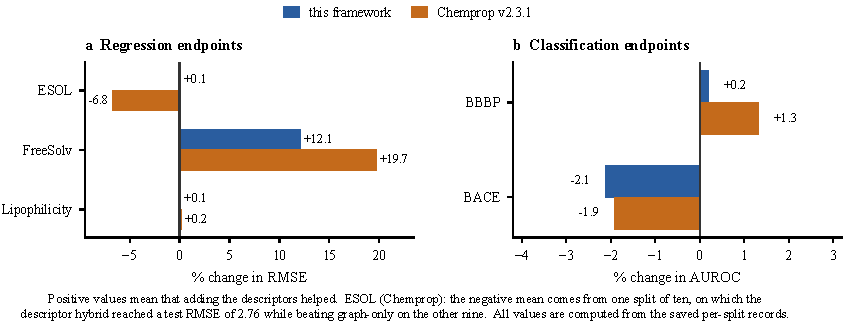
\includegraphics[width=150mm]{figs/fig3_descriptor_effect.pdf}
\caption{Effect of adding 210 RDKit descriptors to a graph-only D-MPNN, in two independently written implementations. Panel (a) shows regression endpoints and panel (b) classification endpoints, so the two metric families are not mixed on one axis. Bars are the change in the ten-split mean of the primary metric (RMSE in (a), AUROC in (b)), signed so that positive values mean lower error or higher AUROC. The ESOL value for Chemprop is dominated by one split, in which its descriptor hybrid reached a test RMSE of 2.76 while being better than graph-only on the other nine; retraining that configuration on that split with six seeds spans 0.75 to 6.12 RMSE, and bounding the descriptor inputs collapses the six retrainings to 0.65--0.72, so the ESOL bar is not an estimate of a stable effect. Computed from Tables~\ref{tab:baselines-regression} and \ref{tab:baselines-classification}.}
\label{fig:descriptor-effect}
\end{figure}

\subsection{Descriptor evidence shows what the data support, not what is universally important}\label{subsec:feature-results}

A chemist approaching a new endpoint asks two things before any model is trained: are the records trustworthy, and which of the several hundred descriptors are actually supported by the training molecules? The audit answers the first, the scorecard and the selectors answer the second, and the two answers are independent of the learner. The audit found duplicated structures in two of the five benchmarks (Table~\ref{tab:hygiene}, discussed below).

Figure~\ref{fig:worked} follows a single molecule through both checks, so that the numbers in the tables can be read on a concrete case.

\begin{figure}[t]
\centering
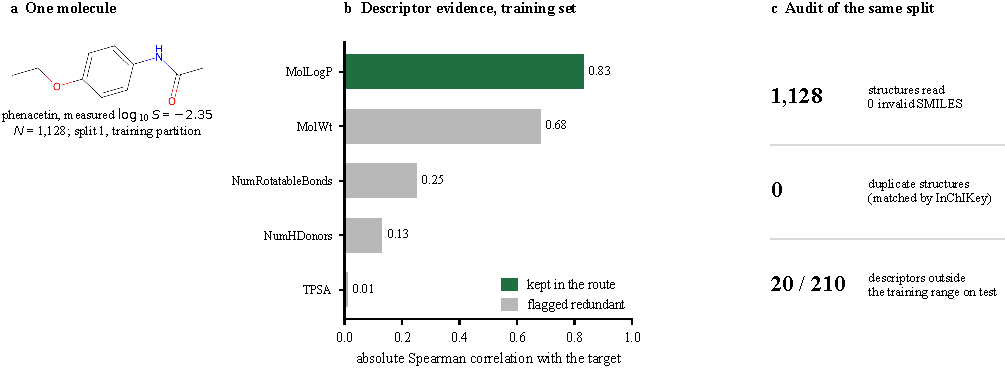
\includegraphics[width=\textwidth]{figs/fig2_worked_example.pdf}
\caption{One molecule followed through the audit and the descriptor scorecard. (a) Phenacetin in the ESOL dataset; its measured aqueous solubility is $\log_{10}S=-2.35$ and it belongs to the training partition of split 1. (b) Training-partition evidence for five of the 210 descriptors. Bars are absolute Spearman correlations with the measured solubility; a descriptor is grey if the recommender did not keep it, which in these cases is because its Pearson correlation with a higher-ranked descriptor exceeded 0.85. (c) Audit output for the same split. The full scorecard covers every descriptor and every split.}
\label{fig:worked}
\end{figure}

With a Random Forest as learner (ESOL, FreeSolv, BBBP), recommended subsets had better mean scores than random subsets of the same size at every budget, and the corrected intervals excluded zero at all budgets on ESOL, at $K\leq20$ on FreeSolv, and at $K=5$ on BBBP; the margin shrank as $K$ grew. At $K=50$ on ESOL, 10 and 20 on FreeSolv, and the three larger budgets on BBBP, the recommendation still had the better mean but the corrected interval did not separate it from random draws. Against the full 210-descriptor pool the picture reverses: at $K=5$ and $K=10$ on ESOL the recommended subset was significantly worse, and every other budget was inconclusive (Additional file 1, Table S4).

A ten-draw control carries its own draw noise, so the comparison was repeated with 50 draws per split and budget in all five endpoints, keeping every draw and testing the recommendation's rank inside the resulting distribution (Additional file 1, Table S5). The recommended subset had the better mean in all 20 dataset--budget cells, and the Fisher-combined rank test was significant in 16: all twelve regression cells ($p\leq1.1\times10^{-3}$; mean percentile $0.88$--$1.00$) and four of the eight classification cells (BBBP at $K=5,10,20$ and BACE at $K=5$, $p=4.4\times10^{-4}$ to $0.036$). The four that did not separate are the larger classification budgets (BBBP $K=50$ and BACE $K=10,20,50$), where a Random Forest on any 50 descriptors already approaches the full-pool AUROC: on BBBP the 50-draw mean is $0.774$ at $K=5$ but $0.905$ at $K=50$, against $0.916$ for the full pool. The advantage of the evidence-based subset is therefore systematic, and largest where descriptors are scarce; it is not a claim that 50 chosen descriptors beat 50 random ones on a classification endpoint.

Across six selectors on five datasets (Table~\ref{tab:selectors}), Random Forest importance and mutual information ranked best on average, with mean ranks of 2.20 and 2.35, respectively. The framework recommender ranked fourth (3.65), was best in one of the 20 dataset-budget cells, and had mean pairwise Jaccard stability of 0.76. This stability was below Spearman ranking (0.88) and mutual information (0.80), but above Random Forest importance (0.65), MI--Pearson (0.57), and L1 (0.47). A Friedman test over the 20 dataset-budget cells rejects equality of the six selectors ($\chi^2=38.3$, $p=3.3\times10^{-7}$), but after Nemenyi correction at $\alpha=0.05$ (critical difference 1.69 ranks) the recommender is not separated from any individual selector, including the best: its gap to Random Forest importance is 1.45 ranks. The individual selector comparisons that survive Holm correction within a dataset are listed in Additional file 1, Table S7. These results support a transparent and reasonably stable candidate-generation heuristic, not a selector that consistently outperforms established alternatives. The selector match with the downstream Random Forest may favour RF importance. Read against the three criteria stated for H1, the 50-draw control meets (i) in all 20 cells on the mean comparison and in 16 on the rank test, the selector comparison fails (ii), and the stability analysis meets (iii).

The practical reading for a chemist is therefore: the scorecard tells you what the data can support, the recommender proposes a compact and stable subset, and the ranking among selectors is close enough that the choice should be made on inspectability and stability rather than on a small score difference.

\begin{table}[t]
\caption{Six feature selectors on five datasets with a Random Forest downstream. Mean rank (1 = best) per dataset over $K\in\{5,10,20,50\}$ and overall over 20 dataset-budget cells; Best denotes cells in which the selector had the best mean score; Jaccard: mean pairwise stability over splits and cells. Full results in Additional file 1, Table S6.}
\label{tab:selectors}
\centering
\footnotesize
\setlength{\tabcolsep}{4pt}
\begin{tabular}{@{}lcccccccc@{}}
\toprule
 & \multicolumn{5}{c}{Mean rank per dataset} & & & \\
\cmidrule(lr){2-6}
Selector & ESOL & FreeSolv & Lipo. & BBBP & BACE & Overall & Best & Jaccard \\
\midrule
RF impurity importance & 1.0 & 1.8 & 1.8 & 4.8 & 1.8 & 2.20 & 10 & 0.65 \\
Mutual information & 2.8 & 2.5 & 1.5 & 2.2 & 2.8 & 2.35 & 3 & 0.80 \\
MI-Pearson & 3.8 & 4.2 & 3.5 & 1.5 & 2.8 & 3.15 & 4 & 0.57 \\
Framework recommender & 3.8 & 3.2 & 3.5 & 3.8 & 4.0 & 3.65 & 1 & 0.76 \\
Spearman top-$K$ & 3.8 & 3.2 & 5.0 & 5.8 & 5.8 & 4.70 & 0 & 0.88 \\
L1 (lasso / L1-logistic) & 6.0 & 6.0 & 5.8 & 3.0 & 4.0 & 4.95 & 2 & 0.47 \\
\bottomrule
\end{tabular}
\end{table}

\subsection{The data audit finds problems that the training score cannot see}\label{subsec:audit-results}

The audit found duplicated structures in two of the five benchmarks (Table~\ref{tab:hygiene}). BBBP contained 64 structures recorded more than once (132 records, 6.5\%), 11 of them with conflicting labels; ESOL contained 11 duplicated structures whose label spans stayed below the conflict threshold (largest span 1.03 log units, compared with a threshold of 1.0478). Across the ten scaffold splits, the mean number of out-of-range descriptors was $19.4\pm12.8$ for ESOL, $20.8\pm14.8$ for Lipophilicity, and $15.1\pm9.5$ for BBBP; the corresponding fractions of test molecules affected were $6.3\pm2.5\%$, $3.7\pm0.7\%$, and $3.8\pm2.1\%$, respectively. These diagnostics are range-based indicators rather than a comprehensive measure of distribution shift. In BBBP the relationship was not monotone: the hybrid's weakest split (split 8) had 19 out-of-range descriptors and 8.8\% of test molecules affected, but split 3 had almost as many (18) and gave the hybrid its best score (Additional file 1, Table S3). A range-based count is therefore a warning flag, not a predictor of which split will be hardest.

\begin{table}[t]
\caption{Structure-level audit by InChIKey. Duplicated structures are structures recorded more than once (records in parentheses). Conflicts are duplicated structures whose labels disagree (classification) or span more than half the target standard deviation (regression).}
\label{tab:hygiene}
\centering
\footnotesize
\begin{tabular}{@{}lrrrrr@{}}
\toprule
Dataset & Records & Unique InChIKeys & Duplicated structures & Conflicts & Largest span \\
\midrule
ESOL & 1,128 & 1,117 & 11 (22) & 0 & 1.03 \\
FreeSolv & 642 & 642 & 0 (0) & 0 & 0.00 \\
Lipophilicity & 4,200 & 4,200 & 0 (0) & 0 & 0.00 \\
BBBP & 2,039 & 1,971 & 64 (132) & 11 & -- \\
BACE & 1,513 & 1,513 & 0 (0) & 0 & -- \\
\bottomrule
\end{tabular}
\end{table}

The duplicate-controlled BBBP sensitivity analysis retained 1,960 unique structures after excluding the 11 conflicting label groups and retaining one record for each of the 53 remaining duplicated groups. On ten new scaffold manifests, mean AUROC was $0.8656\pm0.0577$ for the framework graph only model and $0.8637\pm0.0422$ for its descriptor hybrid. Chemprop v2.3.1 achieved $0.8686\pm0.0398$ with graph only and $0.8744\pm0.0428$ with the 210 molecular descriptors, while RDKit 2D plus Random Forest achieved $0.8940\pm0.0305$ (Additional file 1, Table S16). The hybrid minus graph mean difference was $-0.0019$ for the framework (5/10 splits favoured the hybrid) and $+0.0057$ for Chemprop (9/10 splits favoured the hybrid). For the framework the paired 95\% $t$ interval included zero, so these results do not establish a conclusive advantage from descriptor augmentation in this workflow. The Chemprop hybrid-minus-graph difference was in the same direction but smaller, and its interval also included zero; after Holm correction within the five sensitivity comparisons neither implementation separates (Additional file 1, Table S17). The exact ranking differed from the primary benchmark. Scores were lower for the learned models on the sensitivity data, but this change cannot be attributed to duplicate leakage alone because both data composition and split manifests differed.

\subsection{Descriptor routing depends on feature budget and endpoint}\label{subsec:routing-results}

The harmonised routing results show that the value of a compact descriptor route depends on the endpoint (Table~\ref{tab:routing}). The full 210-descriptor hybrid had the lowest mean RMSE on ESOL ($0.614\pm0.039$) and FreeSolv ($1.038\pm0.214$). On Lipophilicity the recommender route had the lowest mean of the six routes ($0.581\pm0.041$), below the full descriptor set ($0.606$); on BACE the graph-only model had the highest mean AUROC ($0.798$), and the six routes spanned only $0.014$, less than the between-split SD. On BBBP every route lay within $0.007$ AUROC of the best. The random-subset control is the important comparator. The recommender beat it on Lipophilicity ($0.581$ versus $0.591$), but was within one SD of it on ESOL ($0.620$ versus $0.631$), FreeSolv ($1.147$ versus $1.149$), BBBP ($0.915$ versus $0.910$) and BACE ($0.797$ versus $0.792$), and every paired recommender-minus-control difference had a Holm-corrected interval that included zero (Additional file~1, Table~S11). The same correction left the Lipophilicity gap to the full descriptor set inconclusive, so the apparent benefit of compactness is not established at this sample size either. A compact route therefore does not appear to require an informed selection rule on these endpoints; what matters is that it is tested rather than assumed. Per-split outputs and checkpoint decisions are archived in the repository; the checkpoint selection rule and result-file inventory are documented in Additional file~1, Table~S18.

\begin{figure}[t]
\centering
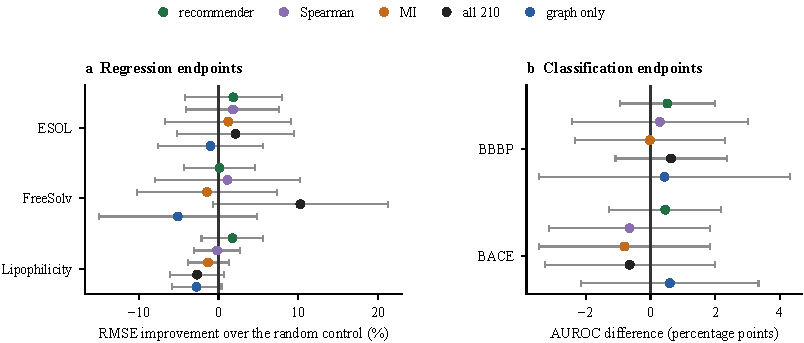
\includegraphics[width=0.92\textwidth]{figs/fig4_routing.pdf}
\caption{Compact descriptor routes compared with the matched random control. Points are mean paired differences over ten splits and error bars are population SDs. Positive values mean that the route had a lower RMSE (a) or a higher AUROC (b) than a random subset of the same size drawn at the same split-specific budget $K^*$. The largest mean improvement is the full descriptor set on FreeSolv (about 10\%), but every interval includes zero: at this sample size no route is separated from its control.}
\label{fig:routing}
\end{figure}

\begin{table}[t]
\caption{Harmonised evidence-guided descriptor routing. Entries are test RMSE for ESOL, FreeSolv, and Lipophilicity, and test AUROC for BBBP and BACE; values are mean $\pm$ population SD over ten saved splits. All route checkpoints are selected by minimum validation loss, and the recommended route's $K^*$ is selected using the primary validation metric at that checkpoint. The random route averages ten random-subset draws per split. Bold text marks the best mean in each row. The two univariate selectors (Spearman and mutual information) are reported in Additional file 1, Table S10, together with the full checkpoint-level audit of 250 model runs (Table S18).}
\label{tab:routing}
\centering
\footnotesize
\setlength{\tabcolsep}{3.2pt}
\begin{tabular}{@{}llcccc@{}}
\toprule
Dataset & Metric & Graph only & All 210 & Recommender & Random \\
ESOL & RMSE $\downarrow$ & $0.638\pm0.074$ & $\mathbf{0.614\pm0.039}$ & $0.620\pm0.078$ & $0.631\pm0.057$ \\
FreeSolv & RMSE $\downarrow$ & $1.205\pm0.164$ & $\mathbf{1.038\pm0.214}$ & $1.147\pm0.140$ & $1.149\pm0.141$ \\
Lipophilicity & RMSE $\downarrow$ & $0.607\pm0.031$ & $0.606\pm0.019$ & $\mathbf{0.581\pm0.041}$ & $0.591\pm0.027$ \\
BBBP & AUROC $\uparrow$ & $0.914\pm0.034$ & $\mathbf{0.916\pm0.029}$ & $0.915\pm0.023$ & $0.910\pm0.020$ \\
BACE & AUROC $\uparrow$ & $\mathbf{0.798\pm0.038}$ & $0.786\pm0.033$ & $0.797\pm0.036$ & $0.792\pm0.042$ \\
\bottomrule
\end{tabular}
\end{table}

\subsection{Configurable predictive roles are useful but not uniformly beneficial}\label{subsec:modularity-results}

The best role assignment was also task dependent (Table~\ref{tab:ablation}). The descriptor-only role was best on ESOL ($0.619$), direct fusion on FreeSolv, Lipophilicity, and BBBP, and graph only on BACE ($0.802$ versus $0.785$ for direct fusion). The margins were often small: on Lipophilicity and ESOL the four learned roles other than the prior and prior-plus-residual variants spanned $0.004$ and $0.018$ RMSE respectively, so the ordering should be read as a trend across ten splits rather than as a separated ranking. No paired interval excluded zero for the prior/residual model against graph only on any task, and on ESOL it had the largest split-to-split variability of the learned models. At the level of training seeds, variation was small relative to split variation for most models (SD over three seeds 0.003 - 0.007 AUROC on BBBP), but reached 0.013 for the prior/residual model, about a third of its between-split SD of 0.034 (Additional file 1, Table S12).

\begin{table}[t]
\caption{Predictive-role ablation (primary metric, mean $\pm$ SD over ten splits; RMSE for ESOL, FreeSolv, and Lipophilicity, AUROC for BBBP and BACE). Bold text marks the best mean per column.}
\label{tab:ablation}
\centering
\footnotesize
\setlength{\tabcolsep}{3pt}
\begin{tabular}{@{}lccccc@{}}
\toprule
Configuration & ESOL & FreeSolv & Lipophilicity & BBBP & BACE \\
\midrule
\cfg{prior\_only} & $0.913\pm0.073$ & $2.015\pm0.116$ & $1.009\pm0.036$ & $0.812\pm0.030$ & $0.660\pm0.055$ \\
\cfg{direct\_only} & $\mathbf{0.619\pm0.045}$ & $1.350\pm0.458$ & $0.683\pm0.034$ & $0.903\pm0.041$ & $0.785\pm0.046$ \\
\cfg{residual\_only} & $0.623\pm0.092$ & $1.251\pm0.153$ & $0.607\pm0.031$ & $0.914\pm0.034$ & $\mathbf{0.802\pm0.038}$ \\
\cfg{direct\_hybrid} & $0.623\pm0.054$ & $\mathbf{1.099\pm0.249}$ & $\mathbf{0.606\pm0.019}$ & $\mathbf{0.916\pm0.029}$ & $0.785\pm0.033$ \\
\cfg{prior\_residual} & $0.681\pm0.113$ & $1.175\pm0.207$ & $0.609\pm0.036$ & $0.910\pm0.034$ & $0.783\pm0.062$ \\
\bottomrule
\end{tabular}
\end{table}

\subsection{Robustness of the inferences}\label{subsec:robustness-results}

Four checks asked whether the conclusions survive a change of statistical view, a change of control protocol, a change of two conventions, and a change of environment.

The primary interval is a Nadeau--Bengio corrected resampled $t$ interval, which is conservative when training sets overlap. Repeating all 184 paired comparisons with an exact sign-flip permutation test, which is computationally exact but makes no overlap correction and is therefore more permissive, reached the same decision in 175 of 184 comparisons and found 23 significant differences rather than 14. The nine disagreements all involve effects whose intervals barely include or exclude zero; none changes a direction, so the conclusions are unchanged when the stricter corrected-interval view is used (Additional file 1, Table S19).

For the routing experiment, none of the 15 route-versus-control comparisons reached significance under the permutation test either (Holm-adjusted $p=1.000$ throughout), so the finding that compact routes are not reliably better than random subsets of the same size does not depend on the interval used.

Two conventions were also varied rather than assumed. Changing the redundancy threshold of the recommender over $0.70$--$0.90$ moved the selected set substantially (mean Jaccard $0.51$--$0.77$ against the default) but changed its downstream score by at most $0.024$ RMSE on ESOL, $0.015$ on FreeSolv and $0.005$ AUROC on BBBP; changing the encoder width over $64$--$256$ kept the sign of the descriptor effect on FreeSolv and changed its size between $7\%$ and $19\%$ (Additional file 1, Tables S20 and S21). In both cases the convention was not what the conclusion depended on.

Finally, because the framework and the Chemprop comparator ran in separate environments with different RDKit releases, the 210-column descriptor block was exported from both and compared cell by cell: 99.87\% of 1{,}999{,}620 cells agree. The differences are confined to ten descriptors, mostly functional-group counts, and are the reason the cross-implementation comparison is described as a replication rather than as an identical-input ablation.

\subsection{The divergent run, diagnosed}\label{subsec:divergence-results}

Two runs in the study departed from every other run of the same configuration, both on ESOL split 3: Chemprop's descriptor hybrid reached a test RMSE of $2.76$ while being better than graph-only on the other nine splits, and the framework's prior/residual route reached $13.23$. Excluding them would have been a post-hoc decision, so both were investigated instead.

Retraining the framework route with three independent training seeds reproduced the failure in all three runs ($13.24$, $13.25$, $13.22$), whereas the direct hybrid on the same split, descriptors and budget gave $0.707$, $0.693$ and $0.727$. The failure is therefore a property of the route and the split, not of one optimisation trajectory. The mechanism is visible in the predicted values: the ridge prior, fitted on the same 50 descriptors, produced test predictions between $-8.09$ and $128.72$ for targets between $-8.40$ and $1.58$, and the residual head adds only a small correction on top of that.

The cause is a single descriptor. \cfg{Ipc} (information content) has a training mean of $2.33\times10^{5}$ and a training SD of $1.70\times10^{6}$ on this split, and the split-3 test set contains a molecule with $\mathrm{Ipc}=5.29\times10^{9}$, which is $3114$ training SDs from the mean. The harness standardises descriptors and replaces infinities by $\pm3$, but it does not bound large finite values, so the network and the ridge prior receive an input of $3113.7$; the largest standardised test value on the other nine ESOL splits is $30.0$. The nonlinear hybrid encoder absorbs this because its descriptor branch is normalised after the first linear layer; the prior/residual route does not, because it adds a linear prediction directly.

Chemprop's hybrid is less stable on the same split. Retraining its archived configuration with six seeds, holding the split, the descriptor block, the model and every hyperparameter fixed, gives test RMSE $0.75$, $1.01$, $1.20$, $2.33$, $5.40$ and $6.12$, with maximum absolute predictions of $8.2$, $9.7$, $12.2$, $24.7$, $50.2$ and $57.2$ against targets spanning $-8.40$ to $1.58$. The archived value of $2.76$ is therefore one draw from an unstable configuration rather than a unique accident: three of the six retrained runs exceed $2.0$ and three stay below $1.3$. Because the archived study trained one seed per split, the Chemprop ESOL descriptor effect of $-6.8\%$ is a property of the seed used on split 3, and we do not interpret its sign; the within-system framework contrast for the same endpoint, which is stable across splits, puts the effect at approximately zero.

The intervention confirms the mechanism. Winsorising the standardised descriptor block at $\pm5$ training standard deviations, with the data, split, model, seeds and all other hyperparameters unchanged, gives $0.666$, $0.699$, $0.719$, $0.698$, $0.653$ and $0.677$ RMSE for the same six seeds: a spread of $0.066$ instead of $5.37$, and a mean of $0.685$ against $2.802$ without the bound. Bounding the magnitude of the descriptor inputs, and nothing else, therefore removes both the tail and the instability. The stabilised hybrid is also close to the graph-only arm on the same split ($0.673$), so once the input is bounded the ESOL descriptor effect is approximately zero rather than negative; the framework's within-system contrast reaches the same conclusion ($+0.1\%$). The failure is a property of the input magnitude, not of Chemprop's training procedure.

The range audit had already flagged the split: ESOL split 3 has 44 of 210 descriptors outside the training range and $11.5\%$ of test molecules affected, more than any other ESOL split. The aggregate count was not sufficient, however, because it does not separate a descriptor one unit beyond the training range from one $3114$ standard deviations beyond it, and Lipophilicity split 9 has more out-of-range descriptors (60) with no divergence. Magnitude separates them: the largest standardised test value on ESOL split 3 is $3114$, against at most $30.0$ on the other nine ESOL splits and at most $62$ on the Lipophilicity splits; the only comparably large values in the audit are BBBP splits 6 and 8 ($430$ and $478$, both on \cfg{Kappa3}), where nothing diverged. A maximum-magnitude check is therefore a warning to inspect rather than a verdict, and we report it in the audit output alongside the range count, with values in the hundreds of training standard deviations treated as a reason to winsorise the descriptor block before interpreting the score.



\section{Discussion}\label{sec:discussion}

The results support an evidence-guided approach to molecular property modelling, rather than a universal ranking of model families. Across five independent endpoints, descriptor-based, graph-based, and hybrid predictors each had tasks on which they performed well. Adding the 210 RDKit descriptors changed performance in the same direction in the framework and Chemprop implementations on four of the five tasks, and by a similar amount: a clear gain on FreeSolv and a change of a few percent or less elsewhere. On ESOL the two disagreed, but only because one Chemprop run diverged: its hybrid was better on nine of ten splits. This cross-implementation agreement, and the single visible failure, support treating descriptor utility as an empirical property of a task and protocol, and as a reason to keep per-split records rather than only summaries.

It is worth stating what this means for the chemist who has one dataset in hand. The default ``use the graph'' or ``use all descriptors'' habit is not wrong, but it is a guess, and the cost of testing it is now small. On phenacetin's endpoint the same graph encoder gave a test RMSE of $0.681$ without descriptors and $0.595$ with them on that split, a difference of $0.086$; averaged over ten splits the graph-only and full-descriptor means are within $0.001$ RMSE of each other on ESOL ($0.623$ versus $0.623$), which is exactly why a single split should not be used as a decision rule. The same holds for compact routes: the recommender gave the lowest mean on Lipophilicity ($0.581$ versus $0.591$ for random subsets), although the paired difference did not survive correction, and it did not separate from the control on any other endpoint. None of these numbers is a universal rule, and the framework deliberately does not turn any of them into one. What it does is make the alternatives cheap enough to compare on the user's own data, with the same split and the same record.

The first contribution is the coupling of feature evidence to model design, with a deliberate distinction between documentation and recommendation. The scorecard is an evidence-documentation and diagnostic layer: it records feature provenance, training support, target association, redundancy, and post-hoc range coverage, while the dataset audit makes duplicate structures and conflicting labels visible. The recommender is a separate candidate-generation heuristic that applies a fixed relevance and redundancy rule; it does not consume categorical scorecard evidence or automatically determine model roles. The recommender was reasonably stable across splits and often improved on random descriptor subsets when a Random Forest was trained directly on the selected descriptors. However, it did not outperform all selectors: Random Forest importance and mutual information ranked higher on average, and the recommender was not reliably superior to random subsets inside graph hybrids. We therefore interpret it as a transparent decision aid, not a new state-of-the-art selector or a measure of universal chemical importance. The scorecard's audit value does not depend on the recommender being the best-performing selector.

The second contribution is a configuration-driven modular architecture. Named feature blocks can be separated from routes and assigned to direct, fixed-prior, or learned-residual roles without changing feature definitions. The role ablation showed why this separation matters: direct fusion had the best mean on three of five tasks and the descriptor-only role on one, while graph only was best on BACE and within $0.001$ RMSE of the best route on Lipophilicity, so the ordering is endpoint-specific and often within between-split noise. The prior and residual design did not produce a statistically conclusive gain over graph only. Its value in this study is therefore architectural flexibility and a controlled way to test role assignments, rather than a claim that this role is consistently more accurate.

The third contribution is evaluation across molecular representations and different prediction endpoints. The same workflow accommodates fingerprints, computed descriptors, graph encoders, and hybrid inputs, and the benchmark spans scalar regression and binary classification. On the duplicate-controlled blood-brain barrier dataset, the framework and Chemprop hybrids had similar mean area under the receiver operating characteristic curve, while the Random Forest on RDKit descriptors had the highest mean. The exact ranking differed from the primary benchmark. Because the cleaned dataset and its split manifests also differed, this sensitivity analysis does not isolate duplicate leakage as the sole cause of the score change. Likewise, the benchmarks are separately trained single-endpoint experiments; they demonstrate cross-task workflow coverage, not the benefit of joint multi-task learning.

Several limitations remain. Ten split manifests still provide limited statistical power for differences of a few hundredths of a metric unit, and overlapping training sets make paired intervals descriptive rather than definitive. The primary blood-brain barrier benchmark retained duplicate structures, including groups with conflicting labels, and the audit found that tautomeric representations can produce different scaffold strings for the same InChIKey. The duplicate-controlled analysis addresses sensitivity to curation, but changes to data composition and splits prevent a causal attribution to leakage alone. Hyperparameters were fixed rather than exhaustively tuned. The descriptor-only reference and the framework's direct descriptor model were produced by different runners. The routing experiment now uses a harmonised checkpoint-selection rule across all five endpoints, with the complete checkpoint-level audit available in the repository. The ten-split summaries are descriptive and should not be interpreted as definitive evidence of small performance differences. Finally, the experiments use two-dimensional inputs and cover only regression and binary classification. Future work should evaluate additional datasets and prospective splits, strengthen duplicate-aware partitioning, test joint multi-task training where supported, and assess whether alternative feature evidence improves decisions beyond the present transparent heuristic.


\section{Conclusions}\label{sec:conclusion}

We stated three hypotheses in the Background so that they could fail. The results answer them as follows.

\emph{H1, evidence is usable: partly supported.} Training-partition evidence is informative enough to act on. With a Random Forest downstream, descriptor subsets chosen from the scorecard beat random subsets of the same size at every budget tested, and the difference survived correction in 8 of the 12 dataset--budget cells. It is not, however, decisive: the recommender ranked fourth of six selectors overall (mean rank 3.65), and the correlation with the target is a weak guide to which descriptors a model will actually use. The honest description is a stable and inspectable way to generate a compact candidate set, not a claim that the selected descriptors are the important ones.

\emph{H2, the descriptor effect transfers: supported on four of five endpoints.} Adding 210 descriptors to a graph model changed the error by a similar amount in two independently written implementations on FreeSolv ($+12.1\%$ and $+19.7\%$), Lipophilicity ($+0.1\%$ and $+0.2\%$), BBBP ($+0.2\%$ and $+1.3\%$) and BACE ($-2.1\%$ and $-1.9\%$). ESOL was the exception, and it is instructive: Chemprop's descriptor hybrid was better than graph-only on nine of ten splits and failed on one (test RMSE 2.76), so the ten-split mean reversed the sign of the effect. A mean without its per-split record would have produced a confident and wrong statement about chemistry. The practical consequence is that a descriptor effect should be reported per split before it is interpreted.

\emph{H3, route and role matter but are endpoint-specific: supported.} The best route differed by endpoint: the full 210-descriptor hybrid on ESOL and FreeSolv, the recommender on Lipophilicity, graph-only on BACE, and no distinguishable winner on BBBP. The best predictive role also changed with the endpoint. Crucially, no compact route separated from a random subset of the same size once paired uncertainty was included, so the route is worth testing but should not be sold as a source of large gains on these endpoints.

Taken together, the three answers point to a practical rule for a chemist: test the alternatives on your own splits, keep the per-split record, and treat a mean that hides one divergent run as unfinished. \framework{} exists to make that rule cheap to follow. An experiment is a plain-text configuration file; the five commands behind it read the data, audit it, validate the configuration, fit the declared representations, and write a record containing the configuration hash, split seed, predictions and checkpoint. A colleague or referee can therefore see which choice was made, on which evidence, and what happened when it was changed. The framework does not promise a universally better predictor, and the results here give no reason to expect one.

\section*{Supplementary information}
\textbf{Additional file 1:} Supplementary results (PDF). Dataset overview, target statistics, and provenance (Table S1a); fixed hyperparameters (Table S1b); scorecard diagnostics and split-level shift analysis (Table S2); recommended versus random subsets and the full pool (Table S3); six-selector results, stability and budget curves (Tables S4 and S4b, Figure S1); internal and external paired comparisons (Tables S5--S6); harmonised descriptor-routing results and their paired comparisons (Tables S7 and S7b); training-seed variance (Table S8); secondary metrics and per-split scores (Tables S9--S10); advisor case study on Caco-2 (Table S11); duplicate-controlled BBBP sensitivity analysis and its paired comparisons (Tables S12 and S12b); checkpoint protocol and result-file inventory (Table S13).

\section*{Abbreviations}
AP, average precision; AUROC, area under the receiver operating characteristic curve; BACE-1, beta-secretase 1; BBBP, blood--brain barrier penetration; CI, confidence interval; D-MPNN, directed message-passing neural network; ECFP, extended-connectivity fingerprint; GIN, graph isomorphism network; GNN, graph neural network; InChI, International Chemical Identifier; InChIKey, International Chemical Identifier key; LARS, least angle regression; MAE, mean absolute error; MI, mutual information; MI-Pearson, selector using mutual-information relevance and Pearson-correlation redundancy; MLP, multilayer perceptron; QSPR, quantitative structure--property relationship; QSAR, quantitative structure--activity relationship; RF, Random Forest; RMSE, root mean squared error; SD, standard deviation; SMILES, simplified molecular input line entry system; TDC, Therapeutics Data Commons.

\section*{Declarations}

\subsection*{Ethics approval and consent to participate}
Not applicable.

\subsection*{Consent for publication}
Not applicable.

\subsection*{Availability of data and materials}
The datasets are publicly available through MoleculeNet \cite{wu2018moleculenet}. Split manifests, configuration files, per-split results, the scripts that produced them, and the manuscript sources are available at \url{https://github.com/soratori1025/Framework-Chemistry} (branch \texttt{paper1}, archived for this submission). Documentation, including a quick-start guide and the configuration reference, is maintained in the same repository.

\subsection*{Competing interests}
The authors declare that they have no competing interests.

\subsection*{Funding}
Not applicable.

\subsection*{Authors' contributions}
D.K.N.N. conceived the framework, developed the software, performed the experiments, analysed the results, and wrote the manuscript.

\subsection*{Acknowledgements}
The author thanks the developers of RDKit, PyTorch, scikit-learn, DeepChem, and Chemprop.

\section{Methods}\label{sec:methods}
% =============================================================================

\subsection{Framework and configuration}\label{subsec:architecture}

\framework{} organises an experiment as data loading, configuration validation, splitting, featurisation, feature analysis, model construction, training, and evaluation (Fig.~\ref{fig:workflow}). Molecules are supplied as strings in the simplified molecular input line entry system (SMILES). A YAML (human-readable data serialisation) configuration declares the input file and targets, named feature blocks, routes that assign blocks to tasks, priors, task types, split strategy, and model, training, evaluation, and analysis settings; it is parsed against a typed schema before any computation. Feature definitions and resolved feature names are hashed, so cached matrices and results can be traced to the definitions that produced them. Feature blocks include element counts, bond-pair counts, substructure counts from SMILES arbitrary target specification (SMARTS) patterns, Morgan fingerprints \cite{rogers2010ecfp}, and the RDKit 2D descriptor set (210 descriptors in RDKit 2023.09.6) \cite{rdkit}; model components, implemented in PyTorch \cite{paszke2019pytorch}, include directed message-passing neural network (D-MPNN) and graph isomorphism network (GIN) encoders, a multilayer perceptron (MLP) descriptor encoder, fusion modules, and task-specific heads. A command-line interface (CLI) and a Python application programming interface (API) expose the commands \cfg{inspect}, \cfg{validate}, \cfg{prepare}, \cfg{train}, and \cfg{predict}. Installation, the configuration reference, and descriptions of every output file are maintained with the source code (\cfg{docs/} and \cfg{README.md} in the repository); the five commands above are also wrapped by a single reproduction script that reruns the benchmark suite. Interfaces for 3D, reaction, mixture, and protein inputs exist but are not evaluated here. The test suite (61 tests) covers configuration parsing, featurisation, feature analysis, the dataset advisor, and training.

% The figure code is kept in fig1_alternatives.tex so that it can also be compiled on
% its own (fig1_preview.tex).  Every number in it comes from
% benchmarks/fig1_worked_example.py.
\subsection{Feature evidence and dataset audit}\label{subsec:feature-evidence}

Training-derived scorecard statistics are computed on the training partition. For each feature the scorecard records provenance, including domain, source and definition, training support (number of molecules with a non-zero value), training mean, standard deviation and range, the Spearman correlation with each target, collinear partners ($|r|\geq0.95$ by default) and, when supplied, bootstrap evidence for prior coefficients and model-dependent group contributions such as permutation or group-removal effects. An ordered rule assigns each feature an evidence class that can be, \emph{out of distribution/unsupported} (zero support or held-out values outside the training range), \emph{weak/uncertain}, \emph{redundant}, \emph{supported} (a sign-consistent prior coefficient whose bootstrap 95\% interval excludes zero, together with a positive model contribution in at least 80\% of repeats) or \emph{model-dependent}. Because the out of distribution class uses held-out ranges, it serves post hoc diagnosis only and is never used for selection; it is a simple range based applicability-domain check \cite{netzeva2005ad,sahigara2012ad}.

The scorecard and recommender serve complementary but distinct purposes. The scorecard is an evidence-documentation and diagnostic layer: it records what is known about a feature under the current dataset and split, but does not itself select features or decide how a feature block enters a model. The recommender is an optional candidate-generation heuristic that returns a compact subset under a fixed relevance and redundancy rule. In particular, the recommender does not consume the scorecard's categorical evidence classes, learn endpoint-specific weights, or automatically alter model architecture. The user remains responsible for deciding whether and how a proposed subset is used.

The dataset advisor (\cfg{inspect}) reports SMILES validity, repeated SMILES strings, scaffold diversity \cite{bemis1996scaffold}, Tanimoto diversity of Morgan fingerprints \cite{rogers2010ecfp,bajusz2015tanimoto}, target skewness, outliers, and class balance, and drafts a starting configuration. For this study, an audit script in the repository additionally matched structures by the International Chemical Identifier key (InChIKey) \cite{heller2015inchi}; a duplicated structure was counted as a conflict if its labels disagreed (classification) or spanned more than half the target standard deviation (regression). Covariate shift between partitions was summarised in two ways: as the number of descriptors with any test value outside the training range and the fraction of test molecules affected, and as the largest standardised test value, obtained by fitting the descriptor standardisation on the training partition and recording the maximum absolute value over the test partition (with the responsible descriptor), together with the number of test molecules exceeding ten training standard deviations. The second summary is reported because a range count treats a value one unit outside the training range and a value thousands of standard deviations outside it identically, and the two have very different consequences for a standardised model input. We report both illustrative split-level diagnostics and the mean and population standard deviation over the ten saved scaffold splits where available. For BBBP, the audit also identified duplicate InChIKeys crossing partition boundaries in several scaffold manifests. Inspection of the affected records showed tautomeric representations that produced different Murcko scaffold strings, so scaffold grouping alone did not guarantee structure identity across partitions.

\subsection{Predictive roles}\label{subsec:roles}

A route maps named feature blocks to a task, so the same block can be reassigned without changing the feature calculator or training loop. In the \emph{direct} role, features are encoded by an MLP and optionally concatenated with the graph representation; in the \emph{prior} role, a feature set $x_p$ defines a baseline fitted on the training partition; in the \emph{residual} role, a network corrects that baseline:
\begin{equation}
    \hat{z}(\mathcal{G}, x_d, x_p) = h_\theta\!\left(\left[\,\phi_\theta(\mathcal{G})\,;\,\psi_\theta(x_d)\,\right]\right) + f_p(x_p),
    \label{eq:prior-residual}
\end{equation}
where $\phi_\theta$ encodes the molecular graph $\mathcal{G}$, $\psi_\theta$ encodes directly routed descriptors $x_d$, $h_\theta$ is the readout and output head, and either encoder can be disabled. For regression $\hat{y}=\hat{z}$; for binary classification $\hat{z}$ is a logit and $\hat{y}=\sigma(\hat{z})$. The pattern follows $\Delta$-machine learning \cite{ramakrishnan2015delta}, with a statistical baseline of physicochemical descriptors in place of a lower-level calculation. The framework fits priors by ridge, least-squares, or logistic regression, optionally with fixed coefficients; in the benchmark, priors were fitted with scikit-learn \cite{pedregosa2011sklearn} (ridge, $\alpha=1$; logistic, $C=1$, using the log-odds from \cfg{decision\_function}) on six descriptors (\cfg{MolWt}, \cfg{MolLogP}, \cfg{TPSA}, \cfg{NumHDonors}, \cfg{NumHAcceptors}, \cfg{NumRotatableBonds}), frozen, and supplied as an input. The network was trained on the original target (Huber loss \cite{huber1964robust} or binary cross-entropy on logits) with AdamW \cite{loshchilov2019adamw}. Listing~\ref{lst:config} shows how roles are declared.

\begin{lstlisting}[float=t, caption={Configuration excerpt showing the three predictive roles in Eq.~\eqref{eq:prior-residual}. The excerpt is validated against the framework schema. Removing the task prior gives a direct hybrid, disabling the descriptor branch gives a prior and residual model, and setting the graph encoder to none gives a descriptor-only model.}, label={lst:config}]
features:
  physchem:                       # six descriptors used by the prior
    type: rdkit_descriptors
    names: [MolWt, MolLogP, TPSA, NumHDonors,
            NumHAcceptors, NumRotatableBonds]
  rdkit2d:                        # full RDKit 2D descriptor pool
    type: rdkit_descriptors
    families: [all]
priors:
  logS_prior: {use: [physchem], fit: ridge}        # prior role
routes:
  logS: [rdkit2d]                                  # direct role
tasks:
  logS: {target: logS, kind: scalar, route: logS, prior: logS_prior}
split: {method: scaffold, fractions: [0.8, 0.1, 0.1], seed: 1}
model:
  structure: {encoder: dmpnn, hidden_dim: 128, depth: 3}   # graph branch
  descriptors: {enabled: true}
  fusion: concat
  prior: frozen
\end{lstlisting}

\subsection{Feature recommendation and comparison selectors}\label{subsec:selectors}

The framework recommendation at budget $K$ (\cfg{select\_evidence\_recommendation}) uses the training partition only: (1) compute the absolute Spearman correlation $s_j$ of each feature with the target, setting $s_j=0$ for features with standard deviation below $10^{-6}$; (2) sort features by $s_j$; (3) add a feature if $s_j\geq10^{-4}$ and its absolute Pearson correlation with every selected feature is at most 0.85; (4) if fewer than $K$ features pass, pad with the next-ranked features. Padding was never triggered: at least 128 descriptors passed step 3 in every split. The rule is a transparent relevance and redundancy heuristic related to correlation based and minimum redundancy selection \cite{hall1999cfs,peng2005mrmr}; it uses the scorecard's association and collinearity statistics but not its evidence classes. It is therefore presented as a reproducible candidate-generation rule for this workflow, not as a novel feature-selection algorithm or a claim that its selected descriptors are universally important.

Five selectors served as comparators at $K\in\{5,10,20,50\}$: Spearman top-$K$; mutual information (MI) top-$K$ with the $k$-nearest-neighbour estimators of scikit-learn ($k=3$) \cite{kraskov2004mi,ross2014mi}; an MI-Pearson selector that greedily maximises mutual information relevance while penalising mean absolute Pearson correlation with selected features; Random Forest impurity importance (100 trees, depth $\leq12$) \cite{breiman2001rf}; and L1 selection, where L1 denotes absolute-value regularisation (order of entry on the least angle regression (LARS) lasso path for regression, or absolute coefficients of an L1-penalised logistic regression with $C=1$ for classification) \cite{tibshirani1996lasso,efron2004lars}. L1 selection used a standard scaler fitted on the training partition only. Random subsets (ten draws per split) and the full pool were additional references on ESOL, FreeSolv, and BBBP. Selected subsets were evaluated with a Random Forest (100 trees). Stability was the mean pairwise Jaccard index of the selected sets over the ten splits \cite{kalousis2007stability,nogueira2018stability}.

\subsection{Evidence-guided descriptor routing}\label{subsec:routing}

To test whether feature evidence can guide model configuration, the 210-descriptor input of the direct hybrid was replaced by a compact route. For each split, the recommended subset was evaluated at $K\in\{10,20,50\}$, and the budget with the best primary validation metric ($K^*$) was retained. Spearman, mutual information (MI), and random subsets reused the same split-specific $K^*$ as matched controls; the random route averaged ten random-subset draws per split. An auxiliary prior and residual model also used the recommended $K^*$ subset as its prior input (\cfg{prior\_rec}); because this changes the predictive role as well as the descriptor route, it is retained in the dataset JSON outputs rather than in the matched direct-hybrid selector table. All compact-route checkpoints were selected by minimum validation loss, and $K^*$ was selected using the primary validation metric evaluated at that checkpoint. The graph-only and full-descriptor references used the same validation-loss checkpoint rule. Thus, checkpoint selection is harmonised across all five datasets and all routing comparisons. The full checkpoint-level audit covers 250 model runs and is recorded in \url{benchmarks/results/routing_checkpoint_audit.csv}; dataset-specific result files are listed in Additional file 1, Table~S18.

\subsection{Datasets and splits}\label{subsec:datasets}

Five datasets from MoleculeNet were used (Table~\ref{tab:datasets}): the ESOL aqueous-solubility benchmark \cite{delaney2004esol}, FreeSolv hydration free energy \cite{mobley2014freesolv}, Lipophilicity \cite{hersey2015lipo}, blood-brain barrier penetration (BBBP) \cite{martins2012bbbp}, and the beta-site amyloid precursor protein cleaving enzyme 1 (BACE-1) inhibition dataset, referred to as BACE \cite{subramanian2016bace}, in their DeepChem distributions \cite{ramsundar2019deep}; SMILES that RDKit could not parse were removed (11 in BBBP), and no deduplication was applied in the primary benchmark. Structures were additionally matched by InChIKey to audit duplicate allocation across the saved partitions. For BBBP, we performed a sensitivity analysis after removing the groups with conflicting labels and retaining one record for each remaining InChIKey. New scaffold split manifests were generated and reused across every model in that sensitivity comparison. Each primary dataset has ten saved 80/10/10 manifests reused by every model. Scaffold splits group molecules by Bemis-Murcko scaffold \cite{bemis1996scaffold}, with acyclic molecules as singleton groups; groups are shuffled with the split seed, sorted by decreasing size, and assigned to the partition whose size is lowest relative to its target fraction. Listing~\ref{lst:split} gives the procedure as executed; the saved manifests, not the code, are what every model consumes. Unlike the DeepChem splitter used for MoleculeNet, large scaffold groups can fall into validation or test, so scores are not directly comparable with published scaffold split values. MoleculeNet recommends random splits for ESOL, FreeSolv, and Lipophilicity \cite{wu2018moleculenet}; we used scaffold splits for ESOL and Lipophilicity to test generalisation beyond the training scaffolds, which is known to be harder but still optimistic relative to prospective use \cite{sheridan2013timesplit,guo2024scaffold}.

\begin{lstlisting}[float=t, language={}, caption={Scaffold partitioning as implemented in \cfg{benchmarks/prepare\_moleculenet\_data.py}. The same seed reproduces the manifest byte for byte; the manifest file, not this code, is the object every model is trained on.}, label={lst:split}]
for seed in 1..10:
    groups  <- molecules grouped by Bemis-Murcko scaffold (acyclic -> singleton)
    groups  <- shuffle(groups, rng(seed))
    groups  <- sort(groups, key = size, descending)
    target  <- (0.8, 0.1, 0.1) * N
    counts  <- (0, 0, 0)
    for g in groups:
        part <- argmin_k( counts[k] / target[k] )
        assign(g, part); counts[part] += size(g)
    save_manifest(seed, train, valid, test)
\end{lstlisting}

\begin{table}[t]
\caption{MoleculeNet datasets, prediction endpoints, primary metrics, and saved split manifests. Counts refer to the processed datasets used in the experiments.}
\label{tab:datasets}
\centering
\scriptsize
\setlength{\tabcolsep}{2.2pt}
\begin{tabular}{@{}p{0.10\textwidth}p{0.19\textwidth}p{0.11\textwidth}p{0.075\textwidth}rrrrp{0.10\textwidth}@{}}
\toprule
Dataset & Endpoint & Task & Metric & $N$ & Train & Valid. & Test & Split \\
\midrule
ESOL & Aqueous solubility ($\log_{10}$ mol\,L$^{-1}$) & Regression & RMSE & 1,128 & 902 & 113 & 113 & Scaffold \\
FreeSolv & Hydration free energy (kcal\,mol$^{-1}$) & Regression & RMSE & 642 & 513 & 64 & 65 & Random \\
Lipophilicity & Octanol/water $\log D$ at pH 7.4 & Regression & RMSE & 4,200 & 3,360 & 420 & 420 & Scaffold \\
BBBP & Blood-brain barrier penetration & Binary class. & AUROC & 2,039 & 1,631 & 204 & 204 & Scaffold \\
BACE & BACE-1 inhibition & Binary class. & AUROC & 1,513 & 1,209 & 152 & 152 & Scaffold \\
\bottomrule
\end{tabular}
\end{table}

The regression targets remain on their native scales. Source-level target summaries, class prevalence, and dataset provenance are provided in Additional file 1, Table S1. The fixed modelling settings are listed in Additional file 1, Table S2.

The five benchmark endpoints were modelled independently. Thus, this study evaluates a common multi-representation workflow across several tasks, rather than joint multi-task learning with parameters shared across multiple endpoints.

\subsection{Reference models and external comparator}\label{subsec:models}

Reference models were a dummy predictor, an extended-connectivity fingerprint with radius 2 and 2,048 bits (ECFP4), RDKit 2D descriptors with a Random Forest (100 trees), and a three-layer descriptor MLP. The external comparator was Chemprop v2.3.1 \cite{graff2026chemprop} (hidden size 300, depth 3, up to 50 epochs with early stopping on validation loss), as a graph-only D-MPNN and with the 210 descriptors as molecule-level features ($x_d$). Five framework configurations isolated feature roles: \cfg{prior\_only}, \cfg{direct\_only} (descriptor MLP), \cfg{residual\_only} (graph only), \cfg{direct\_hybrid} (graph plus 210 descriptors), and \cfg{prior\_residual} (frozen six-descriptor prior plus graph residual). Feature scalers, target scalers, and priors were fitted on training data only; hyperparameters were fixed a priori (Additional file 1, Table S2).

\subsection{Evaluation and statistical analysis}\label{subsec:evaluation}

The primary metrics were test root mean squared error (RMSE) for regression and area under the receiver operating characteristic curve (AUROC) for binary classification. Secondary metrics were mean absolute error (MAE), coefficient of determination ($R^2$), and average precision (AP), and per-split primary scores are given alongside them in Additional file 1 (Tables S13 and S14). Results are means and population standard deviations (SDs) over ten splits. Because methods share splits, comparisons use paired differences $\Delta_s=m_A(s)-m_B(s)$, summarised by their mean, standard deviation, win count, and a 95\% confidence interval (CI) based on a $t$ distribution with nine degrees of freedom. Overlapping training sets make such intervals optimistic \cite{nadeau2003inference,dietterich1998tests}, so they are read descriptively, without multiplicity correction, and an interval that includes zero is treated as inconclusive rather than as equivalence \cite{ash2025comparison}. Training-seed variance was estimated by repeating four configurations with three seeds on one BBBP split.

Three distribution-free checks accompany the intervals. First, every paired comparison was also tested by an exact sign-flip permutation test over the ten splits (all $2^{10}$ sign assignments enumerated, two-sided), with Holm correction inside the same comparison families; the permutation test does not assume normality, but like the naive $t$ test it treats splits as exchangeable and is therefore reported as a secondary, more permissive view rather than as a replacement for the corrected interval. Second, the six selectors were compared as a randomised block design with dataset--budget cells as blocks: a Friedman omnibus test, mean ranks, and a Nemenyi critical difference at $\alpha=0.05$ \cite{demsar2006statistical}. Third, the recommender was compared with random subsets using 50 independent draws per split and budget in every dataset, and the recommender's rank within that distribution was converted to a per-split $p$-value (resolution $1/51$) and combined across splits with Fisher's method \cite{fisher1932statistical}; this replaces the earlier comparison with a ten-draw mean, which carried the draw noise of the control.

Because the framework and the Chemprop comparator ran in different environments, the descriptor block was exported from both and compared cell by cell (\cfg{benchmarks/diagnose\_descriptor\_contract.py}). The two matrices agreed in 99.87\% of 1{,}999{,}620 cells; the differences were confined to ten descriptors, mostly functional-group counts (\cfg{fr\_unbrch\_alkane}, \cfg{fr\_prisulfonamd}, \cfg{NumHAcceptors}) and a small number of BCUT2D, \cfg{SPS} and \cfg{AvgIpc} values whose definitions or implementations changed between RDKit releases. The two implementations therefore saw effectively the same descriptor block, but not a bit-identical one; this is one reason the cross-implementation comparison is read as an independent replication of the descriptor effect rather than as an identical-input ablation.

No run was excluded from any table. The two runs that departed from their configuration, both on ESOL split 3, were diagnosed instead (\cfg{benchmarks/diagnose\_esol\_divergence.py}). The protocol had three parts: (i) describe the descriptor shift of every split in standardised units, (ii) retrain the affected route with additional training seeds, holding the split, descriptors, budget and all hyperparameters fixed (three seeds for the framework route, six for the Chemprop configuration), and (iii) rerun the Chemprop configuration with the standardised descriptor block winsorised at $\pm5$ training standard deviations, for the same six seeds. The third part is an intervention: if the divergence disappears when only the magnitude of the descriptor inputs is bounded, the cause is the input rather than the optimisation. All values in the main tables come from the original runs; the replications are used only to characterise the failure.

\subsection{Sensitivity analyses}\label{subsec:sensitivity}

Two settings are conventions rather than quantities estimated from the data: the redundancy threshold of the greedy pruning step ($0.85$) and the encoder width of the routing experiments ($128$). Each was varied one factor at a time, with everything else fixed, and neither variation was used to choose the configuration reported in the main tables. The redundancy threshold was varied over $0.70$--$0.90$ with $K=20$ fixed, on ESOL, FreeSolv and BBBP, and the overlap between the selected sets was measured with the Jaccard index against the default threshold (Additional file 1, Table S20). Encoder width was varied over $64$, $128$ and $256$ on FreeSolv splits 1--3, retraining the graph-only and direct-hybrid arms from scratch (Additional file 1, Table S21). These analyses test whether a conclusion survives a defensible change of a setting; they do not establish that any setting is optimal.

% =============================================================================


\begin{thebibliography}{99}

\bibitem{todeschini2009descriptors}
Todeschini R, Consonni V. \emph{Molecular descriptors for chemoinformatics}. 2nd ed. Weinheim: Wiley-VCH; 2009. \url{https://doi.org/10.1002/9783527628766}

\bibitem{moriwaki2018mordred}
Moriwaki H, Tian YS, Kawashita N, Takagi T. Mordred: a molecular descriptor calculator. \emph{Journal of Cheminformatics}. 2018;10:4. \url{https://doi.org/10.1186/s13321-018-0258-y}

\bibitem{rogers2010ecfp}
Rogers D, Hahn M. Extended-connectivity fingerprints. \emph{Journal of Chemical Information and Modeling}. 2010;50(5):742--754. \url{https://doi.org/10.1021/ci100050t}

\bibitem{gilmer2017mpnn}
Gilmer J, Schoenholz SS, Riley PF, Vinyals O, Dahl GE. Neural message passing for quantum chemistry. In: \emph{Proceedings of the 34th International Conference on Machine Learning}. PMLR; 2017. p. 1263--1272.

\bibitem{yang2019dmpnn}
Yang K, Swanson K, Jin W, Coley C, Eiden P, Gao H, et al. Analyzing learned molecular representations for property prediction. \emph{Journal of Chemical Information and Modeling}. 2019;59(8):3370--3388. \url{https://doi.org/10.1021/acs.jcim.9b00237}

\bibitem{xu2019gin}
Xu K, Hu W, Leskovec J, Jegelka S. How powerful are graph neural networks? In: \emph{International Conference on Learning Representations}; 2019.

\bibitem{wieder2020review}
Wieder O, Kohlbacher S, Kuenemann M, Garon A, Ducrot P, Seidel T, et al. A compact review of molecular property prediction with graph neural networks. \emph{Drug Discovery Today: Technologies}. 2020;37:1--12. \url{https://doi.org/10.1016/j.ddtec.2020.11.009}

\bibitem{wu2018moleculenet}
Wu Z, Ramsundar B, Feinberg EN, Gomes J, Geniesse C, Pappu AS, et al. MoleculeNet: a benchmark for molecular machine learning. \emph{Chemical Science}. 2018;9:513--530. \url{https://doi.org/10.1039/C7SC02664A}

\bibitem{huang2021tdc}
Huang K, Fu T, Gao W, Zhao Y, Roohani Y, Leskovec J, et al. Therapeutics Data Commons: machine learning datasets and tasks for drug discovery and development. In: \emph{Proceedings of the Neural Information Processing Systems Track on Datasets and Benchmarks}; 2021. \url{https://arxiv.org/abs/2102.09548}

\bibitem{mayr2018largescale}
Mayr A, Klambauer G, Unterthiner T, Steijaert M, Wegner JK, Ceulemans H, et al. Large-scale comparison of machine learning methods for drug target prediction on ChEMBL. \emph{Chemical Science}. 2018;9:5441--5451. \url{https://doi.org/10.1039/C8SC00148K}

\bibitem{jiang2021gnn}
Jiang D, Wu Z, Hsieh CY, Chen G, Liao B, Wang Z, et al. Could graph neural networks learn better molecular representation for drug discovery? A comparison study of descriptor-based and graph-based models. \emph{Journal of Cheminformatics}. 2021;13:12. \url{https://doi.org/10.1186/s13321-020-00479-8}

\bibitem{deng2023systematic}
Deng J, Yang Z, Wang H, Ojima I, Samaras D, Wang F. A systematic study of key elements underlying molecular property prediction. \emph{Nature Communications}. 2023;14:6395. \url{https://doi.org/10.1038/s41467-023-41948-6}

\bibitem{heid2024chemprop}
Heid E, Greenman KP, Chung Y, Li SC, Graff DE, Vermeire FH, et al. Chemprop: a machine learning package for chemical property prediction. \emph{Journal of Chemical Information and Modeling}. 2024;64(1):9--17. \url{https://doi.org/10.1021/acs.jcim.3c01250}

\bibitem{bender2022guidelines}
Bender A, Schneider N, Segler M, Walters WP, Engkvist O, Rodrigues T. Evaluation guidelines for machine learning tools in the chemical sciences. \emph{Nature Reviews Chemistry}. 2022;6(6):428--442. \url{https://doi.org/10.1038/s41570-022-00391-9}

\bibitem{fourches2010trust}
Fourches D, Muratov E, Tropsha A. Trust, but verify: on the importance of chemical structure curation in cheminformatics and QSAR modeling research. \emph{Journal of Chemical Information and Modeling}. 2010;50(7):1189--1204. \url{https://doi.org/10.1021/ci100176x}

\bibitem{shahlaei2013descriptor}
Shahlaei M. Descriptor selection methods in quantitative structure--activity relationship studies: a review study. \emph{Chemical Reviews}. 2013;113(10):8093--8103. \url{https://doi.org/10.1021/cr3004339}

\bibitem{danishuddin2016descriptors}
Danishuddin, Khan AU. Descriptors and their selection methods in QSAR analysis: paradigm for drug design. \emph{Drug Discovery Today}. 2016;21(8):1291--1302. \url{https://doi.org/10.1016/j.drudis.2016.06.013}

\bibitem{khan2018featureselection}
Khan PM, Roy K. Current approaches for choosing feature selection and learning algorithms in quantitative structure--activity relationships (QSAR). \emph{Expert Opinion on Drug Discovery}. 2018;13(12):1075--1089. \url{https://doi.org/10.1080/17460441.2018.1542428}

\bibitem{sheridan2013timesplit}
Sheridan RP. Time-split cross-validation as a method for estimating the goodness of prospective prediction. \emph{Journal of Chemical Information and Modeling}. 2013;53(4):783--790. \url{https://doi.org/10.1021/ci400084k}

\bibitem{butina1999clustering}
Butina D. Unsupervised data base clustering based on Daylight's fingerprint and Tanimoto similarity: a fast and automated way to cluster small and large data sets. \emph{Journal of Chemical Information and Computer Sciences}. 1999;39(4):747--750. \url{https://doi.org/10.1021/ci9803381}

\bibitem{guo2024scaffold}
Guo Q, Hernandez-Hernandez S, Ballester PJ. Scaffold splits overestimate virtual screening performance. In: \emph{Artificial Neural Networks and Machine Learning -- ICANN 2024}. Lecture Notes in Computer Science. Cham: Springer; 2024. \url{https://arxiv.org/abs/2406.00873}

\bibitem{dietterich1998tests}
Dietterich TG. Approximate statistical tests for comparing supervised classification learning algorithms. \emph{Neural Computation}. 1998;10(7):1895--1923. \url{https://doi.org/10.1162/089976698300017197}

\bibitem{nadeau2003inference}
Nadeau C, Bengio Y. Inference for the generalization error. \emph{Machine Learning}. 2003;52:239--281. \url{https://doi.org/10.1023/A:1024068626366}

\bibitem{demsar2006statistical}
Dem\v{s}ar J. Statistical comparisons of classifiers over multiple data sets. \emph{Journal of Machine Learning Research}. 2006;7:1--30.

\bibitem{fisher1932statistical}
Fisher RA. \emph{Statistical Methods for Research Workers}. 4th ed. Edinburgh: Oliver and Boyd; 1932.

\bibitem{ash2025comparison}Ash JR, Wognum C, Rodr\'\i guez-P\'erez R, Aldeghi M, Cheng AC, Clevert DA, et al. Practically significant method comparison protocols for machine learning in small molecule drug discovery. \emph{Journal of Chemical Information and Modeling}. 2025;65(18):9398--9411. \url{https://doi.org/10.1021/acs.jcim.5c01609}

\bibitem{oecd2007guidance}
OECD. Guidance document on the validation of (quantitative) structure--activity relationship [(Q)SAR] models. OECD Series on Testing and Assessment No.~69. Paris: OECD; 2007.

\bibitem{tropsha2010best}
Tropsha A. Best practices for QSAR model development, validation, and exploitation. \emph{Molecular Informatics}. 2010;29(6--7):476--488. \url{https://doi.org/10.1002/minf.201000061}

\bibitem{cherkasov2014qsar}
Cherkasov A, Muratov EN, Fourches D, et al. QSAR modeling: where have you been? Where are you going to? \emph{Journal of Medicinal Chemistry}. 2014;57(12):4977--5010. \url{https://doi.org/10.1021/jm4004285}

\bibitem{netzeva2005ad}
Netzeva TI, Worth A, Aldenberg T, et al. Current status of methods for defining the applicability domain of (quantitative) structure--activity relationships. \emph{Alternatives to Laboratory Animals}. 2005;33(2):155--173. \url{https://doi.org/10.1177/026119290503300209}

\bibitem{sahigara2012ad}
Sahigara F, Mansouri K, Ballabio D, Mauri A, Consonni V, Todeschini R. Comparison of different approaches to define the applicability domain of QSAR models. \emph{Molecules}. 2012;17(5):4791--4810. \url{https://doi.org/10.3390/molecules17054791}

\bibitem{wilkinson2016fair}
Wilkinson MD, Dumontier M, Aalbersberg IJ, et al. The FAIR Guiding Principles for scientific data management and stewardship. \emph{Scientific Data}. 2016;3:160018. \url{https://doi.org/10.1038/sdata.2016.18}

\bibitem{barker2022fair4rs}
Barker M, Chue Hong NP, Katz DS, Lamprecht AL, Martinez-Ortiz C, Psomopoulos F, et al. Introducing the FAIR Principles for research software. \emph{Scientific Data}. 2022;9:622. \url{https://doi.org/10.1038/s41597-022-01710-x}

\bibitem{heil2021reproducibility}
Heil BJ, Hoffman MM, Markowetz F, Lee SI, Greene CS, Hicks SC. Reproducibility standards for machine learning in the life sciences. \emph{Nature Methods}. 2021;18:1132--1135. \url{https://doi.org/10.1038/s41592-021-01256-7}

\bibitem{artrith2021best}
Artrith N, Butler KT, Coudert FX, Han S, Isayev O, Jain A, et al. Best practices in machine learning for chemistry. \emph{Nature Chemistry}. 2021;13:505--508. \url{https://doi.org/10.1038/s41557-021-00716-z}

\bibitem{schuh2026audit}
Schuh MG, Daniluk A, Sieber SA. Auditing widely used biomolecular benchmarks reveals systematic data inconsistencies. \emph{Chemical Science}. 2026;17:17455--17467. \url{https://doi.org/10.1039/D6SC01799A}

\bibitem{guyon2003introduction}
Guyon I, Elisseeff A. An introduction to variable and feature selection. \emph{Journal of Machine Learning Research}. 2003;3:1157--1182.

\bibitem{kraskov2004mi}
Kraskov A, St\"ogbauer H, Grassberger P. Estimating mutual information. \emph{Physical Review E}. 2004;69:066138. \url{https://doi.org/10.1103/PhysRevE.69.066138}

\bibitem{ross2014mi}
Ross BC. Mutual information between discrete and continuous data sets. \emph{PLoS ONE}. 2014;9(2):e87357. \url{https://doi.org/10.1371/journal.pone.0087357}

\bibitem{hall1999cfs}
Hall MA. Correlation-based feature selection for machine learning [PhD thesis]. Hamilton: University of Waikato; 1999.

\bibitem{peng2005mrmr}
Peng H, Long F, Ding C. Feature selection based on mutual information: criteria of max-dependency, max-relevance, and min-redundancy. \emph{IEEE Transactions on Pattern Analysis and Machine Intelligence}. 2005;27(8):1226--1238. \url{https://doi.org/10.1109/TPAMI.2005.159}

\bibitem{tibshirani1996lasso}
Tibshirani R. Regression shrinkage and selection via the lasso. \emph{Journal of the Royal Statistical Society: Series B}. 1996;58(1):267--288. \url{https://doi.org/10.1111/j.2517-6161.1996.tb02080.x}

\bibitem{efron2004lars}
Efron B, Hastie T, Johnstone I, Tibshirani R. Least angle regression. \emph{Annals of Statistics}. 2004;32(2):407--499. \url{https://doi.org/10.1214/009053604000000067}

\bibitem{breiman2001rf}
Breiman L. Random forests. \emph{Machine Learning}. 2001;45:5--32. \url{https://doi.org/10.1023/A:1010933404324}

\bibitem{strobl2007bias}
Strobl C, Boulesteix AL, Zeileis A, Hothorn T. Bias in random forest variable importance measures: illustrations, sources and a solution. \emph{BMC Bioinformatics}. 2007;8:25. \url{https://doi.org/10.1186/1471-2105-8-25}

\bibitem{kursa2010boruta}
Kursa MB, Rudnicki WR. Feature selection with the Boruta package. \emph{Journal of Statistical Software}. 2010;36(11):1--13. \url{https://doi.org/10.18637/jss.v036.i11}

\bibitem{kalousis2007stability}
Kalousis A, Prados J, Hilario M. Stability of feature selection algorithms: a study on high-dimensional spaces. \emph{Knowledge and Information Systems}. 2007;12(1):95--116. \url{https://doi.org/10.1007/s10115-006-0040-8}

\bibitem{nogueira2018stability}
Nogueira S, Sechidis K, Brown G. On the stability of feature selection algorithms. \emph{Journal of Machine Learning Research}. 2018;18(174):1--54.

\bibitem{graff2026chemprop}
Graff DE, Morgan NK, Burns JW, Doner AC, Li B, Li SC, et al. Chemprop v2: an efficient, modular machine learning package for chemical property prediction. \emph{Journal of Chemical Information and Modeling}. 2026;66(1):28--33. \url{https://doi.org/10.1021/acs.jcim.5c02332}

\bibitem{ramakrishnan2015delta}
Ramakrishnan R, Dral PO, Rupp M, von Lilienfeld OA. Big data meets quantum chemistry approximations: the $\Delta$-machine learning approach. \emph{Journal of Chemical Theory and Computation}. 2015;11(5):2087--2096. \url{https://doi.org/10.1021/acs.jctc.5b00099}

\bibitem{aouichaoui2023gcgnn}
Aouichaoui ARN, Fan F, Mansouri SS, Abildskov J, Sin G. Combining group-contribution concept and graph neural networks toward interpretable molecular property models. \emph{Journal of Chemical Information and Modeling}. 2023;63(3):725--744. \url{https://doi.org/10.1021/acs.jcim.2c01091}

\bibitem{ramsundar2019deep}
Ramsundar B, Eastman P, Walters P, Pande V. \emph{Deep learning for the life sciences}. Sebastopol, CA: O'Reilly Media; 2019.

\bibitem{correia2024deepmol}
Correia J, Capela J, Rocha M. DeepMol: an automated machine and deep learning framework for computational chemistry. \emph{Journal of Cheminformatics}. 2024;16:136. \url{https://doi.org/10.1186/s13321-024-00937-7}

\bibitem{mervin2024qsartuna}
Mervin LH, Voronov A, Kabeshov M, Engkvist O. QSARtuna: an automated QSAR modeling platform for molecular property prediction in drug design. \emph{Journal of Chemical Information and Modeling}. 2024;64(14):5365--5374. \url{https://doi.org/10.1021/acs.jcim.4c00457}

\bibitem{dixon2016autoqsar}
Dixon SL, Duan J, Smith E, Von Bargen CD, Sherman W, Repasky MP. AutoQSAR: an automated machine learning tool for best-practice quantitative structure--activity relationship modeling. \emph{Future Medicinal Chemistry}. 2016;8(15):1825--1839. \url{https://doi.org/10.4155/fmc-2016-0093}

\bibitem{vandenmaagdenberg2024qsprpred}
van den Maagdenberg HW, \v{S}\'\i cho M, Araripe DA, et al. QSPRpred: a flexible open source quantitative structure--property relationship modelling tool. \emph{Journal of Cheminformatics}. 2024;16:128. \url{https://doi.org/10.1186/s13321-024-00908-y}

\bibitem{turon2023zairachem}
Turon G, Hlozek J, Woodland JG, Kumar A, Chibale K, Duran-Frigola M. First fully-automated AI/ML virtual screening cascade implemented at a drug discovery centre in Africa. \emph{Nature Communications}. 2023;14:5736. \url{https://doi.org/10.1038/s41467-023-41512-2}

\bibitem{chen2023integrated}
Chen G, Song Z, Qi Z, Sundmacher K. A scalable and integrated machine learning framework for molecular properties prediction. \emph{AIChE Journal}. 2023;69(10):e18185. \url{https://doi.org/10.1002/aic.18185}

\bibitem{yadan2019hydra}
Yadan O. Hydra -- a framework for elegantly configuring complex applications. GitHub; 2019. \url{https://github.com/facebookresearch/hydra}

\bibitem{zaharia2018mlflow}
Zaharia M, Chen A, Davidson A, et al. Accelerating the machine learning lifecycle with MLflow. \emph{IEEE Data Engineering Bulletin}. 2018;41(4):39--45.

\bibitem{rdkit}
RDKit: open source cheminformatics. Version 2023.09.6. \url{https://www.rdkit.org}

\bibitem{paszke2019pytorch}
Paszke A, Gross S, Massa F, et al. PyTorch: an imperative style, high-performance deep learning library. In: \emph{Advances in Neural Information Processing Systems}. 2019;32:8024--8035.

\bibitem{bemis1996scaffold}
Bemis GW, Murcko MA. The properties of known drugs. 1. Molecular frameworks. \emph{Journal of Medicinal Chemistry}. 1996;39(15):2887--2893. \url{https://doi.org/10.1021/jm9602928}

\bibitem{bajusz2015tanimoto}
Bajusz D, R\'acz A, H\'eberger K. Why is Tanimoto index an appropriate choice for fingerprint-based similarity calculations? \emph{Journal of Cheminformatics}. 2015;7:20. \url{https://doi.org/10.1186/s13321-015-0069-3}

\bibitem{heller2015inchi}
Heller SR, McNaught A, Pletnev I, Stein S, Tchekhovskoi D. InChI, the IUPAC International Chemical Identifier. \emph{Journal of Cheminformatics}. 2015;7:23. \url{https://doi.org/10.1186/s13321-015-0068-4}

\bibitem{pedregosa2011sklearn}
Pedregosa F, Varoquaux G, Gramfort A, Michel V, Thirion B, Grisel O, et al. Scikit-learn: machine learning in Python. \emph{Journal of Machine Learning Research}. 2011;12:2825--2830.

\bibitem{huber1964robust}
Huber PJ. Robust estimation of a location parameter. \emph{Annals of Mathematical Statistics}. 1964;35(1):73--101. \url{https://doi.org/10.1214/aoms/1177703732}

\bibitem{loshchilov2019adamw}
Loshchilov I, Hutter F. Decoupled weight decay regularization. In: \emph{International Conference on Learning Representations}; 2019.

\bibitem{delaney2004esol}
Delaney JS. ESOL: estimating aqueous solubility directly from molecular structure. \emph{Journal of Chemical Information and Computer Sciences}. 2004;44(3):1000--1005. \url{https://doi.org/10.1021/ci034243x}

\bibitem{mobley2014freesolv}
Mobley DL, Guthrie JP. FreeSolv: a database of experimental and calculated hydration free energies, with input files. \emph{Journal of Computer-Aided Molecular Design}. 2014;28(7):711--720. \url{https://doi.org/10.1007/s10822-014-9747-x}

\bibitem{hersey2015lipo}
Hersey A. ChEMBL deposited data set -- AZ dataset. 2015. \url{https://doi.org/10.6019/CHEMBL3301361}

\bibitem{martins2012bbbp}
Martins IF, Teixeira AL, Pinheiro L, Falcao AO. A Bayesian approach to in silico blood--brain barrier penetration modeling. \emph{Journal of Chemical Information and Modeling}. 2012;52(6):1686--1697. \url{https://doi.org/10.1021/ci300124c}

\bibitem{subramanian2016bace}
Subramanian G, Ramsundar B, Pande V, Denny RA. Computational modeling of $\beta$-secretase 1 (BACE-1) inhibitors using ligand based approaches. \emph{Journal of Chemical Information and Modeling}. 2016;56(10):1936--1949. \url{https://doi.org/10.1021/acs.jcim.6b00290}
\end{thebibliography}

\end{document}
